\subsection{Ball}

Ball recognition was based on previous code. The main difference is that we don't have to deal with the upclose ball situation. Instead we have to be able to see the ball at an elevated position and with additional glare shining off the ball. A confidence system is used to decide the ball. Confidence is weighted based on correct pixel to size ratio, size and circle fit.

\subsubsection{Ball Distance, Bearing and Elevation Calculations}
The raw values of bearing and elevation are calculated using the centre x and centre y of the blob in the image, while the raw
distance is calculated using the width of the blob in pixels. These resulting values are relative to the camera. They are then transformed using the forward kinematics of the robot to give a relative location in terms of the robots reference frame.

\subsubsection{Circle Fitting}

Least squares circle fitting has been implemented to improve the distances, bearings and elevations of balls that are not fully
visible in the image. There are two main parts to the circle fitting procedure. Firstly the selection of the points to be fit, followed by the fitting of a circle to these points. These points are gathered during one of various scan types depending on the positioning of the ball in the image. The points are found by searching from the outside of the blob inwards until it finds pixels of the same colour of the blob, or in the case of the orange blobs also one of the soft colours close to orange. The directions for which scans have been created are: \emph{Left to Right, Right to Left, Top to Bottom, Bottom to Top,Simultaneous Left to centre \& Right to centre and Simultaneous Top to Centre \& Bottom to Centre}. These can be seen in Figure~{\ref{fig:objectBall3}. The reason the different scanning directions are needed is so that in images in which the view of the ball is cut off by the edge of the image, points are not selected along the edge of the image in turn biasing the circle fit. For more information on the least squares fitting function used see \cite{Seysener2003},\cite{SeysenerMurchMiddleton2004}.

\begin{figure}[!ht]
\begin{center}
    %\leavevmode
    \scalebox{0.3} {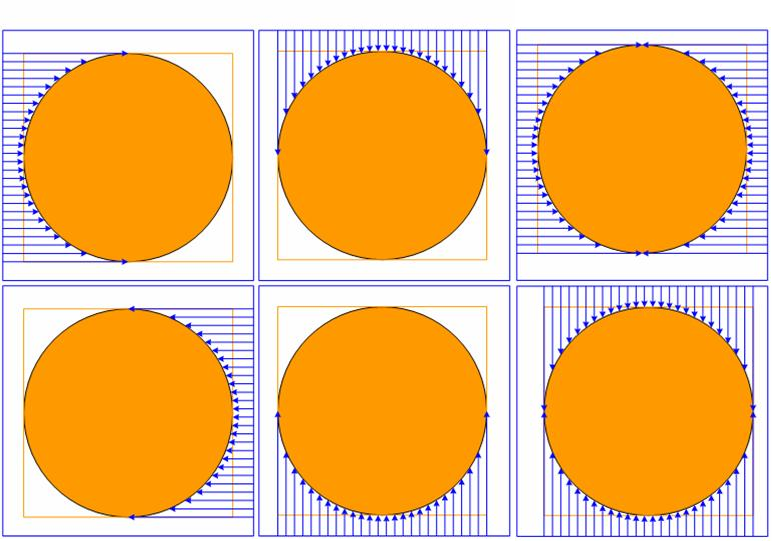
\includegraphics{stevenfigs/objectBall3.png} }
    \caption{Ball scanning directions,  (top left) left to right, (middle left) right to left, (bottom left) left and right to centre, (top right)  top to bottom, (middle right) bottom to top, (bottom right) top and bottom to centre.}
    \label{fig:objectBall3}
\end{center}
\end{figure}

Once a circle has been fit to these points, the validity of the fit circle is determined. If the diameter of the circle is significantly lower that the width of the blob then it is assumed that the circle fit is not correct.


\subsection{Goals}

With the use of soft colour classification and due to obstructions on the field, the goal is often not seen as a single blob, but rather a cluster of blobs. A scan method was used on clusters to detect the gap type and calculate the width of posts.

Gap types are: no gap (unknown post), left (right post), right (left post), middle (both posts, no crossbar), bottom (both posts and crossbar) or undefined. 

Three main variables were used to calculate goal confidence. Correct pixel to size ratio, cluster height to width ratio and goal gap detected.

 
\subsubsection{Goal Distance, Bearing and Elevation Calculations}

The raw distance of the goal is found by using the width of a post. With the new tall goals and the robot camera position looking down for a ball, the goal height is unreliable. If both goal posts are seen both widths are used to calculate the distance to each post. 

The raw bearing and elevation are found using the centre of the post. The method to find the center of the post varies depending on the gap type. As with the ball these raw distances are translated back so they are relative to the hips of the robot. The elevation is not very reliable as the top of the post is often not seen.

\subsubsection{Robots}

Red robots are detected by clusters of red blobs.




